% Author: Justin Yang (typeset by Jaimyn Drake)
% Email: TODO
% Fall 2025

\qns{Have fun periodically!}

\meta{\begin{itemize}
        \item The goal of this problem is just to get comfortable with representing vectors/functions as discrete-periodic signals, and vice versa.
    \end{itemize}
}

% \textbf{Learning Goal:} The goal of this problem is to get practice with inner products, norms and determining orthonormality with complex vectors. 

Recall the following definition of discrete-periodic signals (from EECS16A Notes):

\begin{ln-define}{Discrete-Periodic Signal}{}
    Discrete periodic signals repeat themselves every $p$ samples. Mathematically, they satisfy: 

    \[ x[n] = x[n+p],  \forall n \in \mathbb{Z} \text{ .} \]

    \vspace{0.2in}

    \begin{itemize}
        \item Such a signal is "$p$-periodic".
        \item The fundamental period $p$ is the minimum value of $p$ for which the signal $x$ is p-periodic.
        \item The fundamental angular frequency of the signal is $\omega_0 = \frac{2\pi}{p}$.
    \end{itemize}
\end{ln-define}

Also recall the vector representation of discrete-periodic signals (also from EECS16A Note):

\begin{ln-define}{Vector Representation of DT Periodic Signal}{}
    A $p$-periodic discrete time signals has $p$ distinct values. 
    Thus we can represent such a signal $x$ with a $p$-dimensional column vector:
    
    $$
    \mathbf{x} = 
    \begin{bmatrix}
        x[0] \\
        x[1] \\
        \vdots \\
        x[p-1]
    \end{bmatrix}
    $$
\end{ln-define}

Consider the discrete-time signal $a$ below: 

\vspace{0.2in}

\begin{center}
    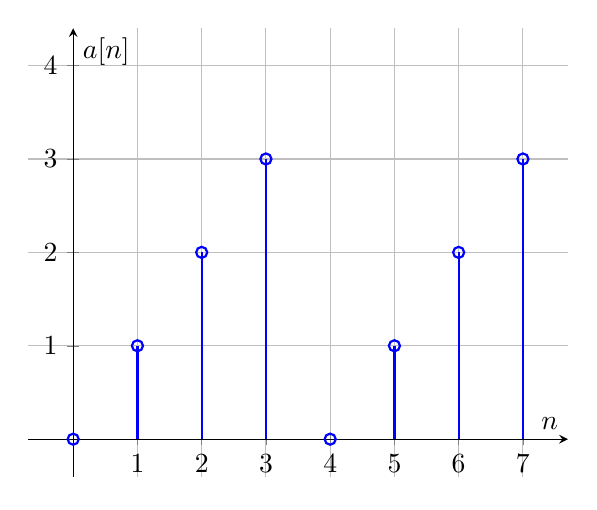
\begin{tikzpicture}
        \begin{axis}[
            axis lines=middle,
            xlabel={$n$},
            ylabel={$a[n]$},
            ymin=0, ymax=4,
            xmin=0, xmax=7,
            xtick={0,1,2,3,4,5,6,7},
            ytick={0,1,2,3,4},
            grid=both,
            enlargelimits=true,
        ]
            \addplot+[
                ycomb,          % This style creates the stems
                mark=o,          % This adds the dots
                thick,
                blue,
            ] coordinates {
                (0, 0) (1, 1) (2, 2) (3, 3) (4, 0) (5, 1) (6, 2) (7, 3)
            };
        \end{axis}
    \end{tikzpicture}
\end{center}

\begin{enumerate}
    \item Find the signal's fundamental period $p$ and vector representation $\mathbf{a}$.

    \ans{
        By inspection, $p = 4$, and $\mathbf{a} = \begin{bmatrix} 0 & 1 & 2 & 3 \end{bmatrix}^ \top$.
    }
    
    \vspace{1in}
\end{enumerate}

% Temporary break out of the enumerate environment
\newcounter{resume_counter}
\setcounter{resume_counter}{\value{enumi}}

Lets play around with transforming $a$ to obtain the target signal:

\begin{center}
    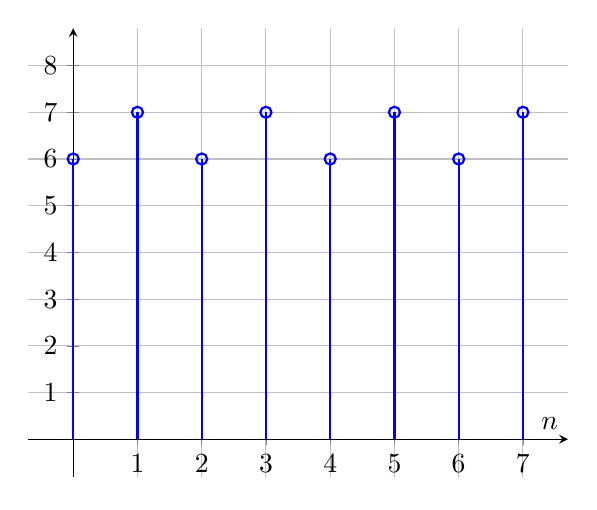
\begin{tikzpicture}
        \begin{axis}[
            axis lines=middle,
            xlabel={$n$},
            ymin=0, ymax=8,
            xmin=0, xmax=7,
            xtick={0,1,2,3,4,5,6,7},
            ytick={0,1,2,3,4,5,6,7,8},
            grid=both,
            enlargelimits=true,
        ]
            % This single command creates the entire stem plot
            \addplot+[
                ycomb,          % This style creates the stems
                mark=o,          % This adds the dots
                thick,
                blue,
            ] coordinates {
                (0, 6) (1, 7) (2, 6) (3, 7) (4, 6) (5, 7) (6, 6) (7, 7)
            };
        \end{axis}
    \end{tikzpicture}
\end{center}

\vspace{0.2in}

For each of the following signals, determine whether or not the signal is periodic. 
If so, find the the signal's fundamental period and vector representation:

\meta{Consider asking student to plot the signals as well, it might make the problem more clear(?)}

\begin{enumerate}
    \setcounter{enumi}{\value{resume_counter}} % Restore the item count

    \item $b[n] = a[-n]$

    \ans{
        \begin{center}
            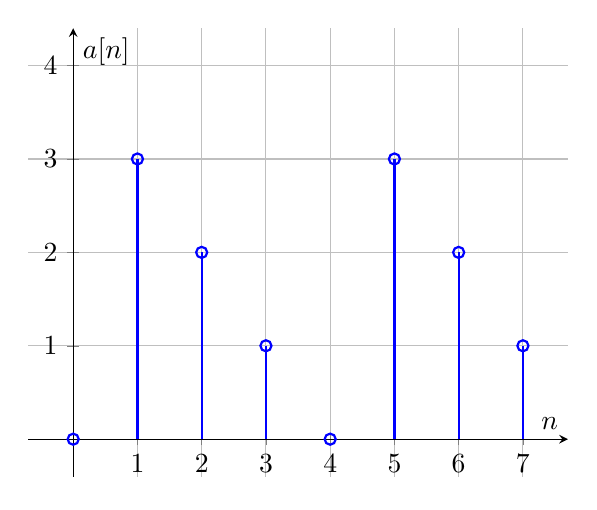
\begin{tikzpicture}
                \begin{axis}[
                    axis lines=middle,
                    xlabel={$n$},
                    ylabel={$a[n]$},
                    ymin=0, ymax=4,
                    xmin=0, xmax=7,
                    xtick={0,1,2,3,4,5,6,7},
                    ytick={0,1,2,3,4},
                    grid=both,
                    enlargelimits=true,
                ]
                    \addplot+[
                        ycomb,
                        mark=o,
                        thick,
                        blue,
                    ] coordinates {
                        (0, 0) (1, 3) (2, 2) (3, 1) (4, 0) (5, 3) (6, 2) (7, 1)
                    };
                \end{axis}
            \end{tikzpicture}
        \end{center}

        \vspace{0.2in}

        Yes, the signal is periodic, $p = 4$, and $\mathbf{b} = \begin{bmatrix} 0 & 3 & 2 & 1 \end{bmatrix}^ \top$. 
    }

    \vspace{1.5in}

    \item $c[n] = b[n+1]$
    
    \ans{
        \begin{center}
            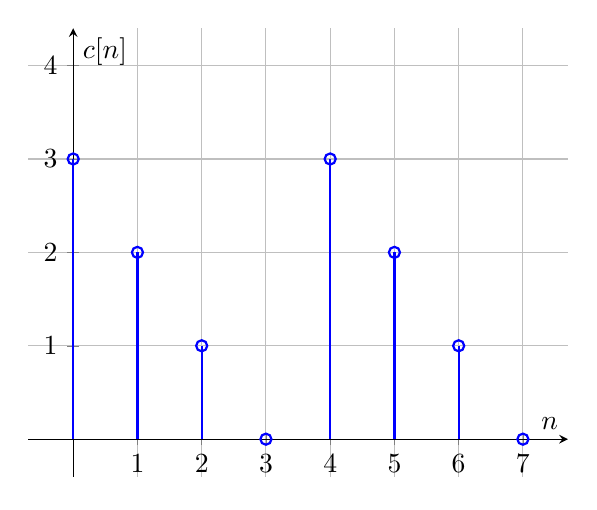
\begin{tikzpicture}
                \begin{axis}[
                    axis lines=middle,
                    xlabel={$n$},
                    ylabel={$c[n]$},
                    ymin=0, ymax=4,
                    xmin=0, xmax=7,
                    xtick={0,1,2,3,4,5,6,7},
                    ytick={0,1,2,3,4},
                    grid=both,
                    enlargelimits=true,
                ]
                    \addplot+[
                        ycomb,
                        mark=o,
                        thick,
                        blue,
                    ] coordinates {
                        (0, 3) (1, 2) (2, 1) (3, 0) (4, 3) (5, 2) (6, 1) (7, 0)
                    };
                \end{axis}
            \end{tikzpicture}
        \end{center}

        \vspace{0.2in}

        Yes, the signal is periodic, $p = 4$, and $\mathbf{c} = \begin{bmatrix} 3 & 2 & 1 & 0 \end{bmatrix}^ \top$. 
    }

    \vspace{1.5in}

    \item $d[n] = \frac{1}{2}(a[n]+a[n-2])$

    \ans{
        \begin{center}
            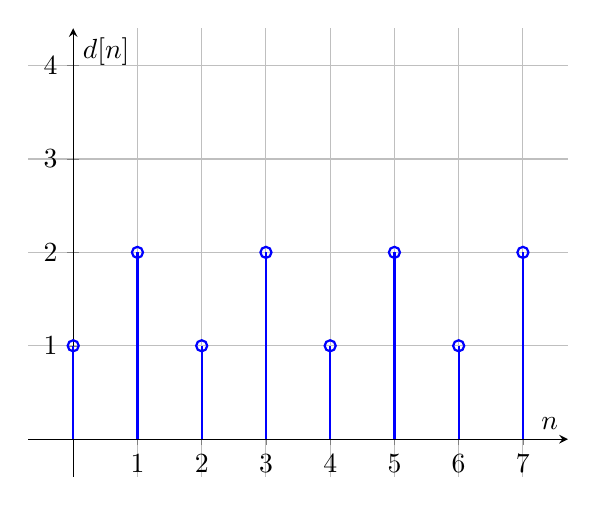
\begin{tikzpicture}
                \begin{axis}[
                    axis lines=middle,
                    xlabel={$n$},
                    ylabel={$d[n]$},
                    ymin=0, ymax=4,
                    xmin=0, xmax=7,
                    xtick={0,1,2,3,4,5,6,7},
                    ytick={0,1,2,3,4},
                    grid=both,
                    enlargelimits=true,
                ]
                    \addplot+[
                        ycomb,
                        mark=o,
                        thick,
                        blue,
                    ] coordinates {
                        (0, 1) (1, 2) (2, 1) (3, 2) (4, 1) (5, 2) (6, 1) (7, 2)
                    };
                \end{axis}
            \end{tikzpicture}
        \end{center}

        \vspace{0.2in}

        Yes, the signal is periodic, $p = 2$, and $\mathbf{d} = \frac{1}{2}\left(\begin{bmatrix} 0 & 1 & 2 & 3 \end{bmatrix}^ \top + \begin{bmatrix} 2 & 3 & 0 & 1 \end{bmatrix}^ \top \right) = \begin{bmatrix} 1 & 2 & 1 & 2 \end{bmatrix}^ \top$. 
    }

    \vspace{1.2in}
    
    \item Finally, find values $A, B, C, D$ to create a linear combination that satisfies:
    \[ Aa[n] + Bb[n] + Cc[n] + Dd[n] = \begin{bmatrix} 6 & 7 & 6 & 7 \end{bmatrix}^ \top \]
    
    \ans{
        \begin{center}
            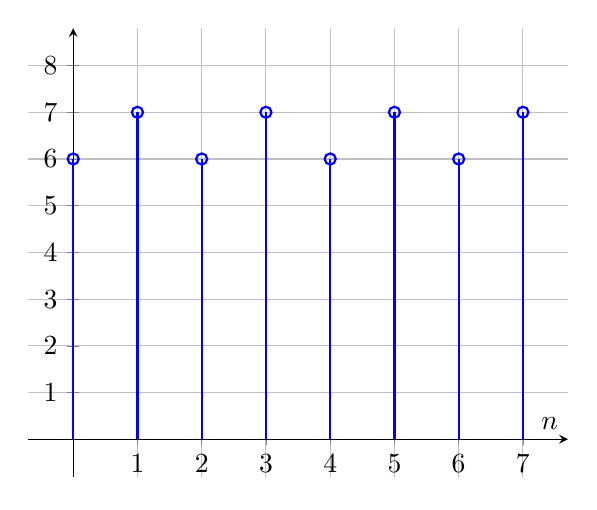
\begin{tikzpicture}
                \begin{axis}[
                    axis lines=middle,
                    xlabel={$n$},
                    ymin=0, ymax=8,
                    xmin=0, xmax=7,
                    xtick={0,1,2,3,4,5,6,7},
                    ytick={0,1,2,3,4,5,6,7,8},
                    grid=both,
                    enlargelimits=true,
                ]
                    % % Plot markers at each stem point
                    % \addplot[mark=o, only marks, blue] coordinates {(-4,1) (-3,1) (-2,1) (-1,1) (0,1) (1,1) (2,1) (3,1) (4,1)};

                    % This single command creates the entire stem plot
                    \addplot+[
                        ycomb,          % This style creates the stems
                        mark=o,          % This adds the dots
                        thick,
                        blue,
                    ] coordinates {
                        (0, 6) (1, 7) (2, 6) (3, 7) (4, 6) (5, 7) (6, 6) (7, 7)
                    };
                \end{axis}
            \end{tikzpicture}
        \end{center}

        \vspace{0.2in}

        The easiest way is to solve this by inspection again.
        Notice that we get a flat/constant signal of value 3 if we add $a$ and $c$: 
        \begin{align*}
            \mathbf{a} + \mathbf{c} &= \begin{bmatrix} 0 & 1 & 2 & 3 \end{bmatrix}^ \top + \begin{bmatrix} 3 & 2 & 1 & 0 \end{bmatrix}^ \top \\
            &= \begin{bmatrix} 3 & 3 & 3 & 3 \end{bmatrix}^ \top
        \end{align*}

        Multiplying by $\frac{5}{3}$ we get $\begin{bmatrix} 5 & 5 & 5 & 5 \end{bmatrix}^ \top$. 
        Then finally adding $\mathbf{d} = \begin{bmatrix} 1 & 2 & 1 & 2 \end{bmatrix}^ \top$ gives us our desired result.
    }

    \vspace{1.5in}

\end{enumerate}
